\documentclass[journal]{vgtc}                % final (journal style)
%\documentclass[review,journal]{vgtc}         % review (journal style)
%\documentclass[widereview]{vgtc}             % wide-spaced review
%\documentclass[preprint,journal]{vgtc}       % preprint (journal style)

%% Uncomment one of the lines above depending on where your paper is
%% in the conference process. ``review'' and ``widereview'' are for review
%% submission, ``preprint'' is for pre-publication, and the final version
%% doesn't use a specific qualifier.

%% Please use one of the ``review'' options in combination with the
%% assigned online id (see below) ONLY if your paper uses a double blind
%% review process. Some conferences, like IEEE Vis and InfoVis, have NOT
%% in the past.

%% Please note that the use of figures other than the optional teaser is not permitted on the first page
%% of the journal version.  Figures should begin on the second page and be
%% in CMYK or Grey scale format, otherwise, colour shifting may occur
%% during the printing process.  Papers submitted with figures other than the optional teaser on the
%% first page will be refused. Also, the teaser figure should only have the
%% width of the abstract as the template enforces it.

%% These few lines make a distinction between latex and pdflatex calls and they
%% bring in essential packages for graphics and font handling.
%% Note that due to the \DeclareGraphicsExtensions{} call it is no longer necessary
%% to provide the the path and extension of a graphics file:
%% 
\includegraphics{diamondrule} is completely sufficient.
%%
\ifpdf%                                % if we use pdflatex
  \pdfoutput=1\relax                   % create PDFs from pdfLaTeX
  \pdfcompresslevel=9                  % PDF Compression
  \pdfoptionpdfminorversion=7          % create PDF 1.7
  \ExecuteOptions{pdftex}
  \usepackage{graphicx}                % allow us to embed graphics files
  \DeclareGraphicsExtensions{.pdf,.png,.jpg,.jpeg} % for pdflatex we expect .pdf, .png, or .jpg files
\else%                                 % else we use pure latex
  \ExecuteOptions{dvips}
  \usepackage{graphicx}                % allow us to embed graphics files
  \DeclareGraphicsExtensions{.eps}     % for pure latex we expect eps files
\fi%

%% it is recomended to use ``\autoref{sec:bla}'' instead of ``Fig.~\ref{sec:bla}''
\graphicspath{{figures/}{pictures/}{images/}{./}} % where to search for the images

\usepackage{microtype}                 % use micro-typography (slightly more compact, better to read)
\PassOptionsToPackage{warn}{textcomp}  % to address font issues with \textrightarrow
\usepackage{textcomp}                  % use better special symbols
\usepackage{mathptmx}                  % use matching math font
\usepackage{times}                     % we use Times as the main font
\renewcommand*\ttdefault{txtt}         % a nicer typewriter font
\usepackage{cite}                      % needed to automatically sort the references
\usepackage{tabu}                      % only used for the table example
\usepackage{booktabs}                  % only used for the table example
%% We encourage the use of mathptmx for consistent usage of times font
%% throughout the proceedings. However, if you encounter conflicts
%% with other math-related packages, you may want to disable it.

%% In preprint mode you may define your own headline.
%\preprinttext{To appear in IEEE Transactions on Visualization and Computer Graphics.}

%% If you are submitting a paper to a conference for review with a double
%% blind reviewing process, please replace the value ``0'' below with your
%% OnlineID. Otherwise, you may safely leave it at ``0''.
\onlineid{0}

%% declare the category of your paper, only shown in review mode
\vgtccategory{Project}
%% please declare the paper type of your paper to help reviewers, only shown in review mode
%% choices:
%% * algorithm/technique
%% * application/design study
%% * evaluation
%% * system
%% * theory/model
\vgtcpapertype{Visulization}

%% Paper title.
\title{Final hand-in for visualization}

%% This is how authors are specified in the journal style

%% indicate IEEE Member or Student Member in form indicated below
\author{Lasse Ahlbech Madsen, Simon Maibom}
\authorfooter{
%% insert punctuation at end of each item
\item
 Lasse Ahlbech Madsen, E-mail: xsc606@alumni.ku.dk
\item
 Simon Maibom: E-mail: xvm226@alumni.ku.dk
}

%other entries to be set up for journal
%\shortauthortitle{Firstauthor \MakeLowercase{\textit{et al.}}: Paper Title}

%% Abstract section.
\abstract{
  Best abstract in the world
} % end of abstract

%% Keywords that describe your work. Will show as 'Index Terms' in journal
%% please capitalize first letter and insert punctuation after last keyword
\keywords{Settlers, Catan, Visualization, Bar charts}

%% ACM Computing Classification System (CCS).
%% See <http://www.acm.org/class/1998/> for details.
%% The ``\CCScat'' command takes four arguments.

\CCScatlist{ % not used in journal version
 \CCScat{K.6.1}{Management of Computing and Information Systems}%
{Project and People Management}{Life Cycle};
 \CCScat{K.7.m}{The Computing Profession}{Miscellaneous}{Ethics}
}

%% Uncomment below to include a teaser figure.
\teaser{
  \centering
  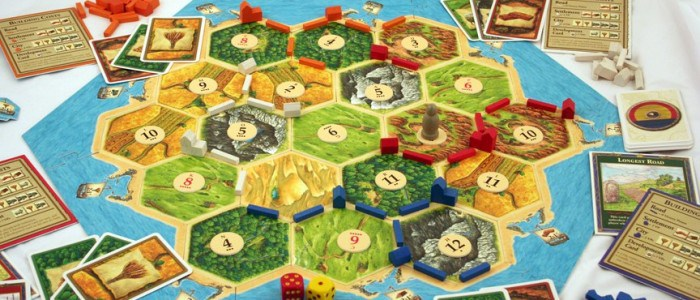
\includegraphics[width=\linewidth]{teaser.jpg}
}

%% Uncomment below to disable the manuscript note
%\renewcommand{\manuscriptnotetxt}{}

%% Copyright space is enabled by default as required by guidelines.
%% It is disabled by the 'review' option or via the following command:
% \nocopyrightspace

\vgtcinsertpkg

%%%%%%%%%%%%%%%%%%%%%%%%%%%%%%%%%%%%%%%%%%%%%%%%%%%%%%%%%%%%%%%%
%%%%%%%%%%%%%%%%%%%%%% START OF THE PAPER %%%%%%%%%%%%%%%%%%%%%%
%%%%%%%%%%%%%%%%%%%%%%%%%%%%%%%%%%%%%%%%%%%%%%%%%%%%%%%%%%%%%%%%%

\begin{document}

%% The ``\maketitle'' command must be the first command after the
%% ``\begin{document}'' command. It prepares and prints the title block.

%% the only exception to this rule is the \firstsection command
\firstsection{Introduction}

\maketitle

We have decided to work with the boardgame Settlers of Catan. The idea is to
visualize the effects of starting choices on the outcome of the game. It is a
game about managing odds and hedging your bets, so frequent players will be
interested in knowing what types of starting locations that gives a high
probability of winning.

\subsection{About the game}

Settlers of Catan is a game where you and a number of other players settle
an island. During the course of the game you acquire resources, build
improvements and acquire points. The first to 10 points wins the game.

For our project it is important to know that a settlement is located next
to 3 resource tiles with a number tile on top. Whenever the dice outcome is
the same as a number of a tile all players next to it receive a resource
token. Settlements can also be located next to the sea where there are harbors
that can be used to trade resources.

\section{Related work}

There have not been much work done on the topic, we have not been able to
find actual visualizations of the game, but we did find one analysis by Peter
Keep\cite{peter}. He attempts to use probabilities to estimate the worth of
resources and getting a gist of an optimal strategy. He never refers to his
dataset, but merely states things as known. He makes a good argument for his
approach to find the value of resources, but in his conclusions he fails to
take rarity of resources fully into account.

\section{Data and Task Abstractions} % BEDRE OVERSKRIFTER

\subsection{Domain Situation}

The target audience of the project is intermediate Settlers of Catan
players, who wants to get better at the game by getting a deeper understanding
of how to place the two starting settlements in order to maximize the chance
to win.

Relevant questions these players might ask would either be very concrete
in-the-moment questions or generally browsing for good combinations and things
to avoid. We imagine most players would be interested in just browsing the
data as well.

\begin{itemize}
  \item "What is the optimal settlement location?"
  \item "Is it best to be in the first spot?"
  \item "Is it feasible to settle without access to all resources?"
  \item "Does settling next to a desert always cause a loss?"
  \item "If my first settlement has wood and ore what resource should I go
    for?"
\end{itemize}

\subsection{Data and Task Abstractions}


The dataset\cite{lumin} consists of data for 50 4-player games. Each game
has 4 lines that consist of starting position, points gained, placements of
starting towns, total resource gains and losses from production, robber cards
and trade.

A snapshot of the dataset can be seen in appendix 1. We have mostly
used the data from the settlements and the points. The types of the attributes
can be seen in table \ref{tab:types}. It is worth nothing that the dices on
the resources are categorical because comparisons of them in this context is
meaningless.

\begin{figure}
  \centering
  \begin{tabular}{|l|l|}
    \hline
    Data & Type \\ \hline
    GameNum & Ratio \\ \hline
    Player & Categorical \\ \hline
    Points & Ratio \\ \hline
    Me & Categorical \\ \hline
    Dice throws & Categorical \\ \hline
    Settlement:res & Categorical \\ \hline
    Settlement:dice & Categorical \\ \hline
    Gains & Ratio\\ \hline
    Losses & Ratio \\ \hline
  \end{tabular}
  \caption{Attribute types}
  \label{tab:types}
\end{figure}

To win a game of Settlers you need 10 points and there will never be two
players with 10 or more points at the same time. However it is possible to
finish the game with 11 or 12 points, but this skews the data without being
particularly interesting when determining a winner, so we changed all values
above 10 to just 10.

Generally points are the main indicator of success in the game, so whenever we
need to analyze the quality of combinations we will measure it against points
and occasionally win-rate.

We did not consider gains and losses all that interesting. They are mostly
based on chance that is dependent on your settlements. We could show them, but
it would merely be a correlation between high gains and winning. The
experience Settler player would not be particularly interested in seeing this.

\section{Design}

Based on our data and task abstractions it would seem that the most important
part is the ability to view probabilities and to search the data for exact
situations. There are too many possible combinations for pie charts and the
probabilities do not relate to each other, so we stuck with simple bar
charts for the main part of our visualization.

What was more important was the filtering of data and we want to ensure that
any scenario can be created. We imagined doing this just with checkboxes, but
we modified this for implementation.

\subsection{Illustration}
\begin{figure}[!h]
  \centering
  
\includegraphics[scale=0.4]{pic2.png}
\end{figure}
\newpage
\noindent

The sketch shows on the left side a bunch of filters that you apply, once the
user have applied the filters on the right side will show a bunch of graphs
of game statistics. These graphs include how many points gained relative to
which number or resource a player had next to the starting settlements and
other relevant statistics. The filters that the user should be able to apply,
includes which player position, how many of a resource the start settlements
border and whether they are next to a desert.

\subsection{Scenario of use}

% OPDATER SCENARIOS
\subsubsection{Scenario 1}
A user wants to know whether it is a good idea to place settlements with no
access to clay. He skims through the list of visualization possibilities
and finds the resources tabs and chooses starts with "At most 0" of a
resource. A bar chart is shown with 5 bars, one for each resource type. He
finds the clay bar and the task is complete.

\section{Implementation}

We implemented the visualization using the D3-library. To make data processing easier,
We used python to transform the settlement columns from a list of a comma separated values seen at fig \ref{tab:data}.
Into four columns with settlement position in one value and rolls on the specific settlement,
for both first and second settlement. All data processing were done using javascript.
%% if specified like this the section will be committed in review mode
\acknowledgments{
The authors wish to thank the Kaggle user "Lumin" for sharing his game stats}

%\bibliographystyle{abbrv}
\bibliographystyle{abbrv-doi}
%\bibliographystyle{abbrv-doi-narrow}
%\bibliographystyle{abbrv-doi-hyperref}
%\bibliographystyle{abbrv-doi-hyperref-narrow}

\bibliography{template}

\appendix
\newpage
\section{Appendix 1: Dataset}

Our dataset consists of 50 games each with 4 players. This makes for 200 lines
of data. In tabel \ref{tab:data} a condensed version of the data can be seen.
There are columns for all dice throws between 2 and 12.

\begin{figure}[h!]
  \centering
  \begin{tabular}{|l|l|l|l|l|l|l|l|l|l|l|l|}
    \hline
    GameNum & Player & Points & Me & 2 & ... & 12 & & & & & \\ \hline
    1 & 1 & 5 & & 1 & ... & 1 & & & & & \\ \hline
    1 & 2 & 9 & 1 & 1 & ... & 1 & & & & & \\ \hline
    1 & 3 & 10 & & 1 & ... & 1 & & & & & \\ \hline
    1 & 4 & 5 & & 1 & ... & 1 & & & & & \\ \hline \hline
    Set1 & & & & & & Set2 & & & & & \\ \hline
    6 & L & 3 & C & 11 & C & 9 & L & 10 & W & 11 & O \\ \hline
    5 & W & 8 & O & 10 & W & 4 & L & 5 & S & 11 & O \\ \hline
    5 & S & 6 & S & 12 & W & 8 & O & 4 & S & 3 & C \\ \hline
    6 & O & 9 & L & 3 & L & 4 & L & 8 & L & 10 & S \\ \hline \hline
    Production & TradeGain & RobberGain & TotalGain & TradeLoss & RobberLoss &
    Tribute & totalLoss & totalAvailable & & & \\ \hline
    38 & 5 & 2 & 45 & 10 & 2 & 4 & 16 & 29 & & & \\ \hline
    48 & 8 & 6 & 62 & 11 & 1 & 8 & 20 & 42 & & & \\ \hline
    44 & 14 & 9 & 67 & 24 & 4 & 0 & 28 & 39 & & & \\ \hline
    42 & 12 & 0 & 54 & 24 & 6 & 0 & 30 & 24 & & & \\ \hline
  \end{tabular}
  \caption{Dataset snapshot}
  \label{tab:data}
\end{figure}



\end{document}

